%This is a template for the University of Helsinki. If you have questions regarding the template please be in contact with uhbrand@helsinki.fi

%This template was designed by Zafar Hussain and Lalli Myllyaho for the Department of Computer Science, University of Helsinki.

\documentclass[final]{beamer}
\mode<presentation>

% STEP 1:
% Please use 'XeLaTex' or 'LuaLaTex' compiler. To select one of them, click on the 'Menu' button in the left corner and select one of the above-mentioned-compiler.

\usepackage[english]{babel}
\usefonttheme{serif}

% This poster is designed for a three-column recommended style. For two or four columns, you will have to change '.sty' files accordingly.
\usepackage[orientation=portrait,size=a0,scale=1.2]{beamerposter}
\usetheme[COM, threecolumn]{HYposter}

%Remember to change the name of .bib file if you have uploaded with a different name

\addbibresource{bibliography.bib}

% STEP 2: Set up the title and author info
\titlestart{TWO WORDS}% First two words are yellow
%To keep title all grey, just comment out the above \titlestart command.
\titleend{ IN ORANGE AND THE REST IN GREY (OR ONLY GREY)} % second line of title
\titlesize{\veryHuge} % Use this to change title size if necessary. possible sizes are 'small', 'large', 'Large', 'LARGE', 'huge','Huge', 'veryHuge', VeryHuge', 'VERYHuge'. 

\author{
  \small Mario Armando, Urbina Silva \\
  \footnotesize{mariosva139@hotmail.com}, \\Escuela de Ciencias Físicas y Matemáticas, \\Universidad de San Carlos de Guatemala}

% Read the docs if you need to add the logo(s) of institutes involved in this work. 
\leftcorner{{
\includegraphics[height=5cm]{img/Imagen2.png}}}

%These are the recommended font styles. If you want to change to something else, you might need to work with the '.sty' files.

\setmainfont{Georgia}
\setsansfont{Arial}

\begin{document}

\begin{poster}

% STEP 3: Add the contents of your poster between \begin{poster} and \end{poster}

% Use the '\newcolumn' command to create a column at a specific place. If the text of a paragraph does not fit into a column, you can use this command to start a new column. 

\newcolumn
\section{HEADLINE IN UPPERCASE}
\justifying
Lorem Ipsum is simply dummy text of the printing and typesetting industry. Lorem Ipsum has been the industry's standard dummy text ever since the 1500s, when an unknown printer took a galley of type and scrambled it to make a type specimen book. It has survived not only five centuries, but also the leap into electronic typesetting, remaining essentially unchanged. It was popularised in the 1960s with the release of Letraset sheets containing Lorem Ipsum passages. uf Zerm hawr rwivos


\section{Heading here}
\justifying
Lorem Ipsum is simply dummy text of the printing and typesetting industry. Lorem Ipsum has been the industry's standard dummy text ever since the 1500s, when an unknown printer took a galley of type and scrambled it to make a type specimen book. 

\begin{figure}
    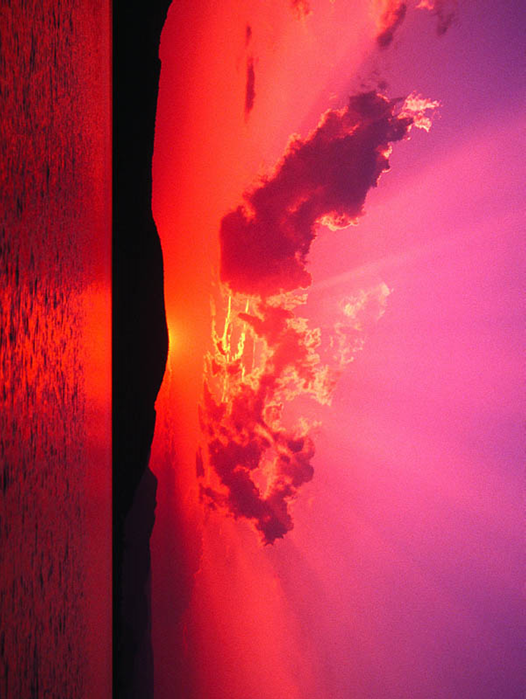
\includegraphics[width=0.99\textwidth]{flames/pic1.png}
    \caption{\sffamily{} Leave some space before and after pictures. The caption can be a text like this.}
    \label{fig:pic1}
\end{figure}

\newcolumn

\section{Another headline}
\justifying
Lorem Ipsum is simply dummy text of the printing and typesetting industry. Lorem Ipsum has been the industry's standard dummy text ever since the 1500s, when an unknown printer took a galley of type and scrambled it to make a type specimen book. 

\begin{itemize}
  \item Hello.
  \item The text in the entries may be of any length.
\end{itemize}

It was popularised in the 1960s with the release of Letraset sheets containing Lorem Ipsum passages, and more recently with desktop publishing software like Aldus PageMaker including versions of Lorem Ipsum.

\begin{figure}
    \centering
    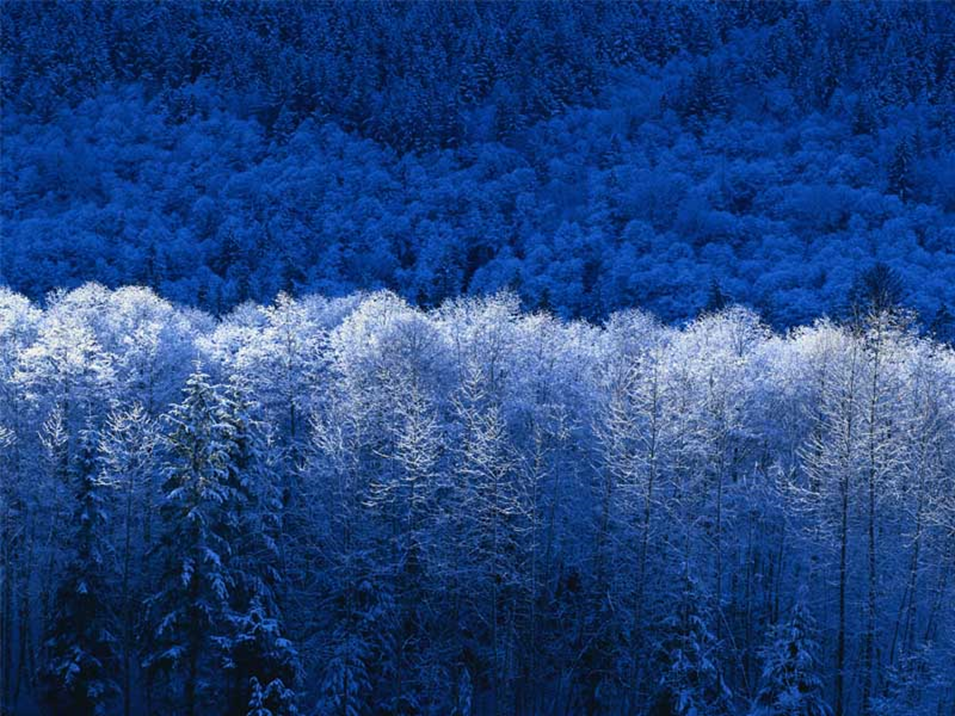
\includegraphics[width=0.99\textwidth]{flames/pic2.png}
    \caption{\sffamily A caption again.}
\end{figure}

Lorem Ipsum is simply dummy text of the printing and typesetting industry. Lorem Ipsum has been the industry's standard dummy text ever since the 1500s, when an unknown printer took a galley of type and scrambled it to make a type specimen book. It has survived not only five centuries, but also the leap into electronic typesetting, remaining essentially unchanged.

\begin{equation*}
R(t)= A \left(\frac{E_0}{\rho_0}\right)^{1/5}t^{2/5}
\end{equation*}

% Third column
\newcolumn
\justifying It has survived not only five centuries but also the leap into electronic typesetting, remaining essentially unchanged. It was popularised in the 1960s with the release of Letraset sheets containing Lorem Ipsum passages, and more recently with desktop publishing software like Aldus PageMaker including versions of Lorem Ipsum.  Let's cite! Einstein's journal paper \cite{einstein} and Dirac's book \cite{dirac} are physics-related items. 

%If you want to add white space between paragraphs or sections, you can use 'vspace{1em}' command. Where you can use number of em accordingly.

\vspace{1em}
\section{Yet another headline}
\justifying
Lorem Ipsum is simply dummy text of the printing and typesetting industry. Lorem Ipsum has been the industry's standard dummy text ever since the 1500s when an unknown printer took a galley of type and scrambled it to make a type specimen book.

\begin{table}
\caption{Example Table}
    \begin{tabular*}{\columnwidth}{@{\extracolsep{\fill}} |c|r|r|r| }
    \hline
        $x$ & $x^2$ & $x^3$ & $x^4$\\
        \hline
        1 &  1 &   1 &   1 \\
        \hline
        2 &  4 &   8 &  16 \\
        \hline
        3 &  9 &  27 &  81 \\
        \hline
        4 & 16 &  64 & 256 \\
        \hline
        5 & 25 & 125 & 625 \\
        \hline
    \end{tabular*}
\end{table}

Lorem Ipsum has been the industry's standard dummy text ever since the 1500s when an unknown printer took a galley of type and scrambled it to make a type specimen book.

\section{References}
\printbibliography[heading=none]

\end{poster}
\end{document}
